\newcommand{\walletcollector}{\texttt{wallet\_collector}}
\newcommand{\userinforetriever}{\texttt{user\_info\_retriever}}
\newcommand{\addresschecker}{\texttt{address\_checker}}
\newcommand{\graph}{\texttt{graph}}

\section{Nduja}
\subsection{High level architecture}
Nduja was developed in Python\footnote{it should be used with Python3.5+} and it
is composed by four main modules, represented in Figure\ref{fig:architecture}:
\begin{enumerate*}[label=\roman*),itemjoin={,\quad}]
\item \walletcollector{} is a set of classes whose aim is to retrieve
addresses of different cryptocurrencies. It provides a different class for each
different sources that we used, following the same interface
\item \userinforetriever{} is a set of classes that, based on which
site a wallet is discovered, retrieve some information (e.g. name, email,
personal website) related to the owner of that wallet
\item \addresschecker{} is a module that have to check if a sequence of
characters recognized as an address is a real and used addresses. For certain
altcoins it is not possible to perform this validation action accurately, e.g.
Monero has private transactions, so it is not possible to find out that
information
\item \graph{} is the module that create graph with which is possible to
correlate addresses and plot graphs.
\end{enumerate*}

\begin{figure}[t]
\centering
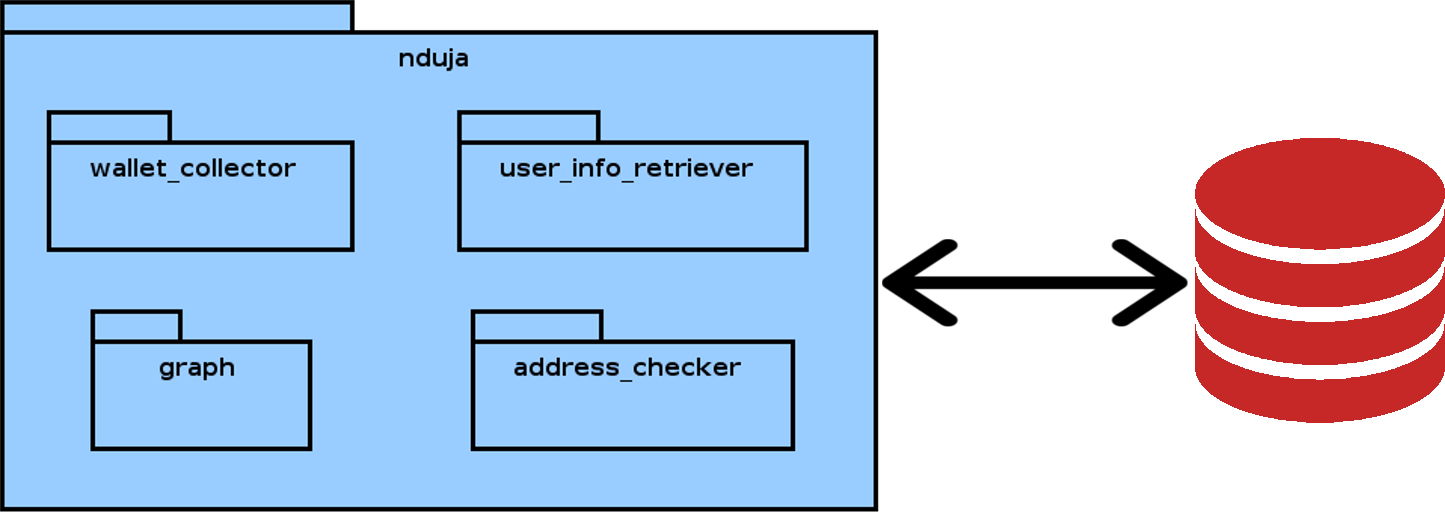
\includegraphics[scale=0.22]{db}
\caption{Nduja high level architecture}
\label{fig:architecture}
\end{figure}

\subsection{Queries} 
\label{sec:queries}
In order to maximize the number of possible results in repositories the module
\walletcollector{} searches for files that contains words such as
\textbf{donation} or \textbf{contribution} and in which there is a set of
characters that matches regular expressions that we defined for different
address formats. This has been implemented using two different APIs: Github
Search API \footnote{\url{https://developer.github.com/v3/search/}} and
Searchcode API \footnote{\url{https://searchcode.com/api/}}.
Instead, in order to query Twitter we looked for the same keywords that in the
repositories but also for \textit{hashtags} such as \textbf{\#GiveAway} or for
hashtags correlated to specific cryptocurrency (e.g. \#BTCGiveAway). This has
been done using Twitter API
\footnote{\url{https://developer.twitter.com/en/docs/api-reference-index}}.
Twitter API has a strong limitation: we are only able to retrieve tweets that
are published at most a week before the search. This limitation is imposed
because we have not paid for a premium account=. In fact our research must be
thought as a proof of concept. Even if you would use a free account you can
collect incremental data doing the query weekly: the information before the
first search is lost without a premium account, but, following this idea you
are able to collect all the future addresses.

\subsection{Database}
All data we have retrieved is stored into a
SQLite\footnote{\url{https://www.sqlite.org/}} database. Addresses are save with
the indication that if they are wallets retrieved from the websites we search,
if they are inferred or they are ``tagged'' addresses. These are wallets that
are known a priori: that means that are used by famous services, such as mixing
services or betting games as
\textit{SatoshiDICE}\footnote{\url{satoshidice.com}}. We excluded that kind of
services from data retrieving process for two reasons: the first is that we did
not want that the number of addresses explode, the latter is that these
addresses are ``public'' yet, so they are useless for the aim of our study.

\subsection{Algorithm}
\texttt{Nduja} algorithm follows a sequence of 3 steps:
\subsubsection*{Data retrieving} Firstly all the possible wallets are collected
and inserted into the database. In order to do this the research on
Twitter and Github and using Searchcode API is performed. The addresses
discovered are stored in relation to the account that advertised them.
\todo{explain difference between Account and Wallet Address throughout the
paper}
In this paper we refer to \textit{Account} when we talk about a Twitter, Github
or some other repositories host profile, instead with \textit{Address} or
\textit{Wallet} we mean the public key of a wallet of a certain cryptocurrency.
\subsubsection*{Account data retrieving} The second steps involves the
retrieving of all possible data related to accounts inserted into the database
in step 1: this is done using related API (e.g. Twitter API, Github Search API,
Bitbucket API, ...) but also searching for emails and websites in the same file
of the addresses.
\subsubsection*{Clustering addresses} The last step consists in grouping 
wallets that could be associated with the same person. In order to do so we
take advantage of
Blockchain.info API\footnote{\url{https://blockchain.info/api}},
Chain.so API\footnote{\url{https://chain.so/api}} and
Etherscan API\footnote{\url{https://etherscan.io/apis}}. These APIs allow
developers to query Bitcoin, Ethereum, Litecoin and Dogecoin blockchains without
having a local copy of the blockchain, that can counts hundreds of
gigabytes~\cite{}\todo{Add citation for this assertion ->
this? \url{https://bitinfocharts.com/}}.
We used them to find out all the transactions regarding a single wallet
in our database. 

After that we looked for transactions with multiple inputs that
involve wallets that we connected to a certain person in order to create a
``cluster'' of wallet of the same user. 

Indeed as already stated by Satoshi Nakamoto~\cite{}:
\begin{quotation}
	As an additional firewall, a new key pair should be used for each
	transaction to keep them from being linked to a common owner.
	Some linking is still unavoidable with multi-input transactions, which
	necessarily reveal that their inputs were owned by the same owner. 
	The risk is that if the owner of a key is revealed, linking could reveal
	other transactions that belonged to
	the same owner.
\end{quotation}
\todo{Move where we start to explain our project?}



TODO Explain better












